\documentclass{article}


\usepackage{arxiv}

\usepackage[utf8]{inputenc} % allow utf-8 input
\usepackage[T1]{fontenc}    % use 8-bit T1 fonts
\usepackage{hyperref}       % hyperlinks
\usepackage{url}            % simple URL typesetting
\usepackage{booktabs}       % professional-quality tables
\usepackage{amsfonts}       % blackboard math symbols
\usepackage{nicefrac}       % compact symbols for 1/2, etc.
\usepackage{microtype}      % microtypography
\usepackage{lipsum}
\usepackage{tikz}
\usepackage{dsfont}
\usepackage{amsmath}
\usepackage{array}
\usepackage{todonotes}
\usepackage{float}
\usepackage{rotating}
\usepackage[toc,page]{appendix} %appendix
%\usepackage[sort&compress,square,comma,authoryear]{natbib}

\definecolor{maroon}{RGB}{176, 48, 96}
\definecolor{orange2}{RGB}{238, 118, 0}
\newcommand{\colindic}[1]{\textcolor{maroon}{#1}}
\newcommand{\colsurvey}[1]{\textcolor{orange2}{#1}}


\title{Pattern of early human-to-human transmission of Wuhan 2019-nCoV}


\author{
   Julien Riou, MD, PhD \\
  Institute of Social and Preventive Medicine\\
  University of Bern\\
  Bern, Switzerland \\
  \texttt{julien.riou@ispm.unibe.ch} \\
  \And
Christian L.~Althaus, PhD \\
Institute of Social and Preventive Medicine\\
University of Bern\\
Bern, Switzerland \\
\texttt{christian.althaus@alumni.ethz.ch}
}



\begin{document}
\maketitle

\begin{abstract}
On December 31, 2019, the World Health Organization was notified about a cluster of pneumonia of unknown aetiology in the city of Wuhan, China. Chinese authorities later identified a new coronavirus (2019-nCoV) as the causative agent of the outbreak. As of January 23, 2020, 650 cases have been confirmed in China and several other countries. Understanding the transmission characteristics and the potential for sustained human-to-human transmission of 2019-nCoV is critically important for coordinating current screening and containment strategies, and determining whether the outbreak constitutes a public health emergency of international concern (PHEIC). We performed stochastic simulations of early outbreak trajectories that are consistent with the epidemiological findings to date. We found the basic reproduction number, $R_0$, to be around 2.2 (90\% high density interval 1.4--3.8), indicating the potential for sustained human-to-human transmission. Transmission characteristics appear to be of a similar magnitude to severe acute respiratory syndrome-related coronavirus (SARS-CoV) and the 1918 pandemic influenza. These findings underline the importance of heightened screening, surveillance and control efforts, particularly at airports and other travel hubs, in order to prevent further international spread of 2019-nCoV.
\end{abstract}

\section*{Introduction}

On December 31, 2019, the World Health Organization (WHO) was alerted about a cluster of pneumonia of unknown aetiology in the city of Wuhan, China\cite{who1}. Only a few days later, Chinese authorities identified and characterised a novel coronavirus (2019-nCoV) as the causative agent of the outbreak \cite{Shi:2020}. The outbreak apparently started from a single or multiple zoonotic transmission events at a wet market in Wuhan, and has since resulted in 654 confirmed cases in China and several other countries by January 23, 2020 \cite{wiki}. At this early stage of the outbreak, it is critically important to gain a better understanding of the transmission pattern and the potential for sustained human-to-human transmission of 2019-nCoV. Information on the transmission characteristics will help coordinate current screening and containment strategies, support decision making on whether the outbreak constitutes a public health emergency of international concern (PHEIC), and is necessary for anticipating the risk of pandemic spread of 2019-nCoV.

Two key properties will determine further spread of 2019-nCoV. First, the basic reproduction number $R_0$ describes the average number of secondary cases generated by an infectious index case during the early phase of the outbreak. If$R_0$ is above the critical threshold of 1, continuous human-to-human transmission with sustained transmission chains will occur. Second, the individual variation in the number of secondary cases provides further information about the early outbreak dynamics and the expected number of superspreading events \cite{Lloyd-Smith:2005,Althaus:2015b,Kucharski:2015b}.

In order to better understand the early transmission pattern of 2019-nCoV, we performed stochastic simulations of early outbreak trajectories that are consistent with the epidemiological findings to date.
%
%
%\cite{Shi:2020}
%
%- Info about outbreak
%- Why it is important to understand transmission characteristics, and why we want to know $k$ and superspreading (limitation of study by Leung).
%
%We used stochastic simulations in order to identify the likely transmission characteristics that have results in the early outbreak trajectory as reported to date.

\section*{Methods}
We performed stochastic simulations of the first few generations of human-to-human transmission of 2019-nCoV. 
Simulations were initialized with one index case.
For each primary case, we generated secondary cases according to a negative-binomial offspring distribution with mean $R_0$ and dispersion $k$.\cite{Lloyd-Smith:2005,Althaus:2015b}
The dispersion parameter $k$ can be interpreted as a measure of the probability of superspreading events (the lower the value of $k$, the higher the probability of superspreading).
The generation time interval $D$ was assumed to be gamma-distributed with a shape parameter of 2, and a mean that varied between 7 and 14 days.
We explored a wide range of parameter combinations (Table \ref{fig:tab1}) and ran 1,000 stochastic simulations for each individual combination. 
This corresponds to a total of 3.52 million one-index-case simulations that were run on UBELIX (\url{http://www.id.unibe.ch/hpc}), the high performance computing cluster at the University of Bern. 

In a second step, we accounted for the uncertainty regarding the number of index cases $n$ and the date $T$ of the initial zoonotic animal-to-human transmissions at the wet market in Wuhan. 
An epidemic with several index cases can be considered as the sum of several independent epidemics with one index case each.
We sampled (with replacement) $n$ of the one-index-case epidemics, sampled a date of onset for each index case, and summed the epidemic curves together.
The sampling of the date of onset was done uniformly from a two-week interval around November 27, 2019, in coherence with early phylogenetic analyses of 11 2019-nCoV genomes.\cite{Rambaut:2020}
This step was repeated 4,800 times for each combination of $R_0$ (22 points) and $k$ (20 points) for a total of 2,112,000 full epidemics simulated that included the uncertainty on $D$, $n$ and $T$.
Finally, we calculated the proportion of stochastic simulations that reached a total number of infected cases within the interval [1000, 9700] by January 18, 2020, as estimated by Imai and colleagues.\cite{Imai:2020}
In a process related to Approximated Bayesian Computation (ABC), the parameter value combinations that led to simulations within that interval were treated as approximations to the posterior distributions of the parameters with uniform prior distributions.
Model simulations and analyses were performed in the R software for statistical computing.\cite{R:2018} 
Code files are available on \url{https://github.com/jriou/wcov}.

\begin{table}
	\centering
	\caption{Parameter ranges for stochastic simulations of outbreak trajectories.}
	\label{fig:tab1}
\begin{tabular}{llll}
	\hline
	Parameter & Description & Range   \\
	\hline 
	$R_0$& Basic reproduction number  &[0.8 -- 5.0] \\ 
	$k$ & Dispersion parameter & [0.01 -- 10] \\
	$D$ & Generation time interval & [7 -- 14]  \\
	$n$ & Initial number of index cases & [1 -- 50]  \\
	$T$ & Date of zoonotic transmission & [20 Nov 2019 -- 4 Dec 2019] \\
	
	\hline 
\end{tabular} 
\end{table}

\section*{Results}
In order to reach between 1,000 and 9,700 infected cases by January 18, 2020, the early human-to-human transmission of 2019-nCoV must be either characterized by values of $R_0$ around around 2.2 (90\% high density interval 1.4--3.8) (figure \ref{fig:fig2}).
Observed data at this point is compatible with a large range of values for the dispersion parameter $k$ (median 0.54, 90\% high density interval 0.014--6.95).
However, our simulations suggest that very low values of $k$, corresponding to a large probability of superspreading events, are less likely.
These estimates incorporate the uncertainty on the current total epidemic size (as of January 23, 2020) and on the date and scale of the initial zoonotic event (figure \ref{fig:fig3}).

Comparison with other emerging viruses in the past allows to put in perspective the available information regarding the transmission patterns of 2019-nCoV.
Our estimates of $R_0$ and $k$ are more similar to previous estimates focusing on early human-to-human transmission of SARS-CoV in Beijing and Singapore\cite{Lloyd-Smith:2005} than of MERS-CoV\cite{Kucharski:2015b} (figure \ref{fig:fig1}).
These estimates are also in line with those of 1918 Influenza.\cite{Fraser:2011}


%([2, 5]) and low values of $k$ (< 1). The latter scenario is similar to what has been estimated for SARS-CoV and indicates the considerable potential for superspreading of 2019-nCoV.

\begin{figure}[h]
	\centering
	\includegraphics[width=.6\linewidth]{../figure/fig2b.pdf}
	\caption{Values of $R_0$ and $k$ most compatible with epidemic data available on 2019-nCoV as of January 23, 2020 (in blue). The basic reproduction number $R_0$ quantifies human-to-human transmission. The dispersion parameter $k$ quantifies the risk of a superspreading event (lower values of $k$ are linked to a higher probability of superspreading).}
	\label{fig:fig2}
\end{figure}


\begin{figure}[h]
	\centering
	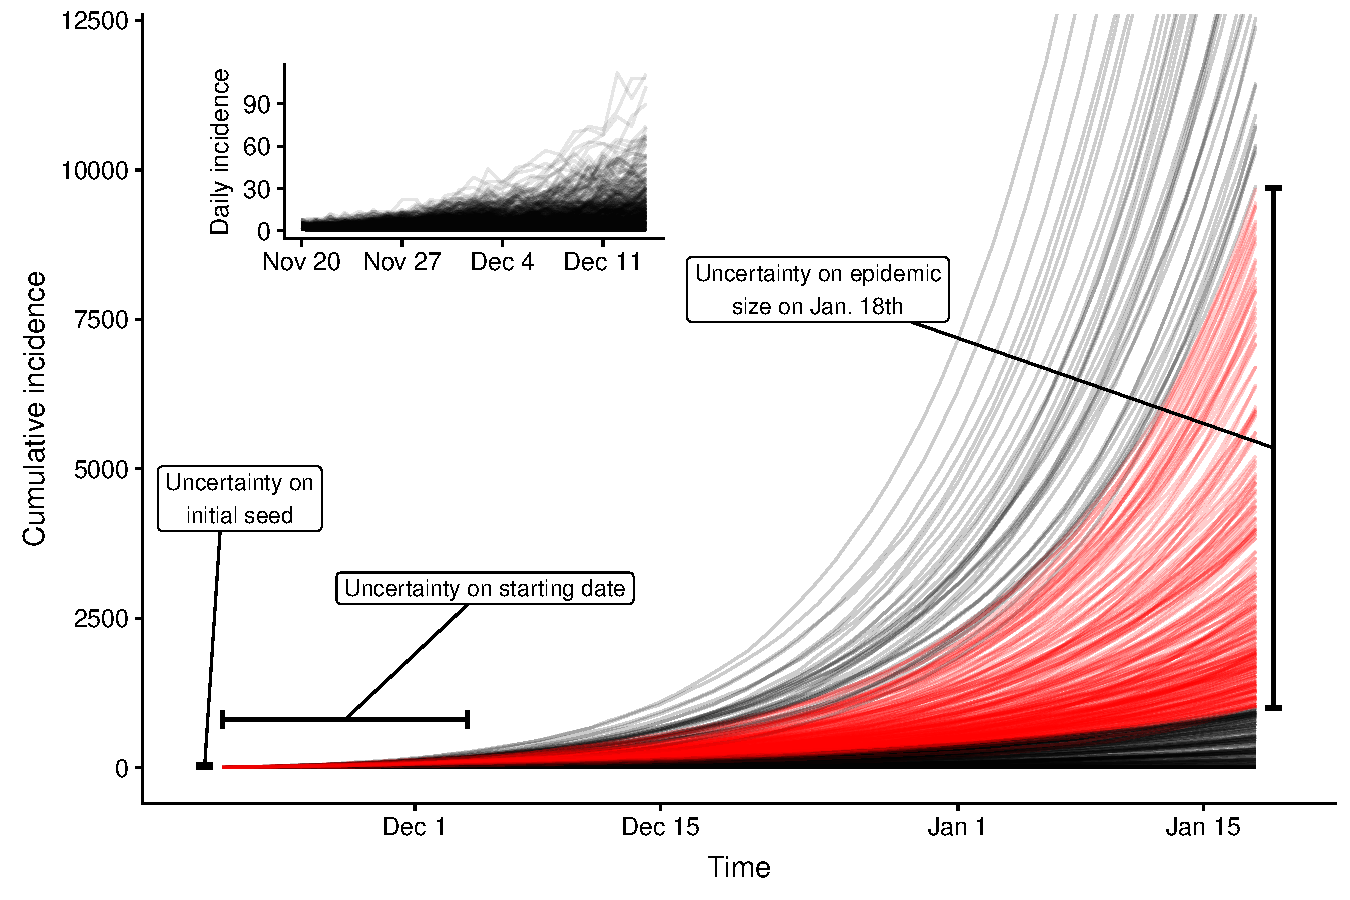
\includegraphics[width=.9\linewidth]{../figure/fig3b.pdf}
	\caption{Illustration of the simulation strategy. The lines represent the cumulative incidence of 100 simulations with $R_0=1.8$ and $k=1.62$. The other parameters are left to vary according to table 1. Among these epidemics, 54.4\% led to a cumulative incidence between 1000 and 9700 on January 18, 2020 (in red, as in figure \ref{fig:fig3}).}
	\label{fig:fig3}
\end{figure}


\begin{figure}[h]
	\centering
	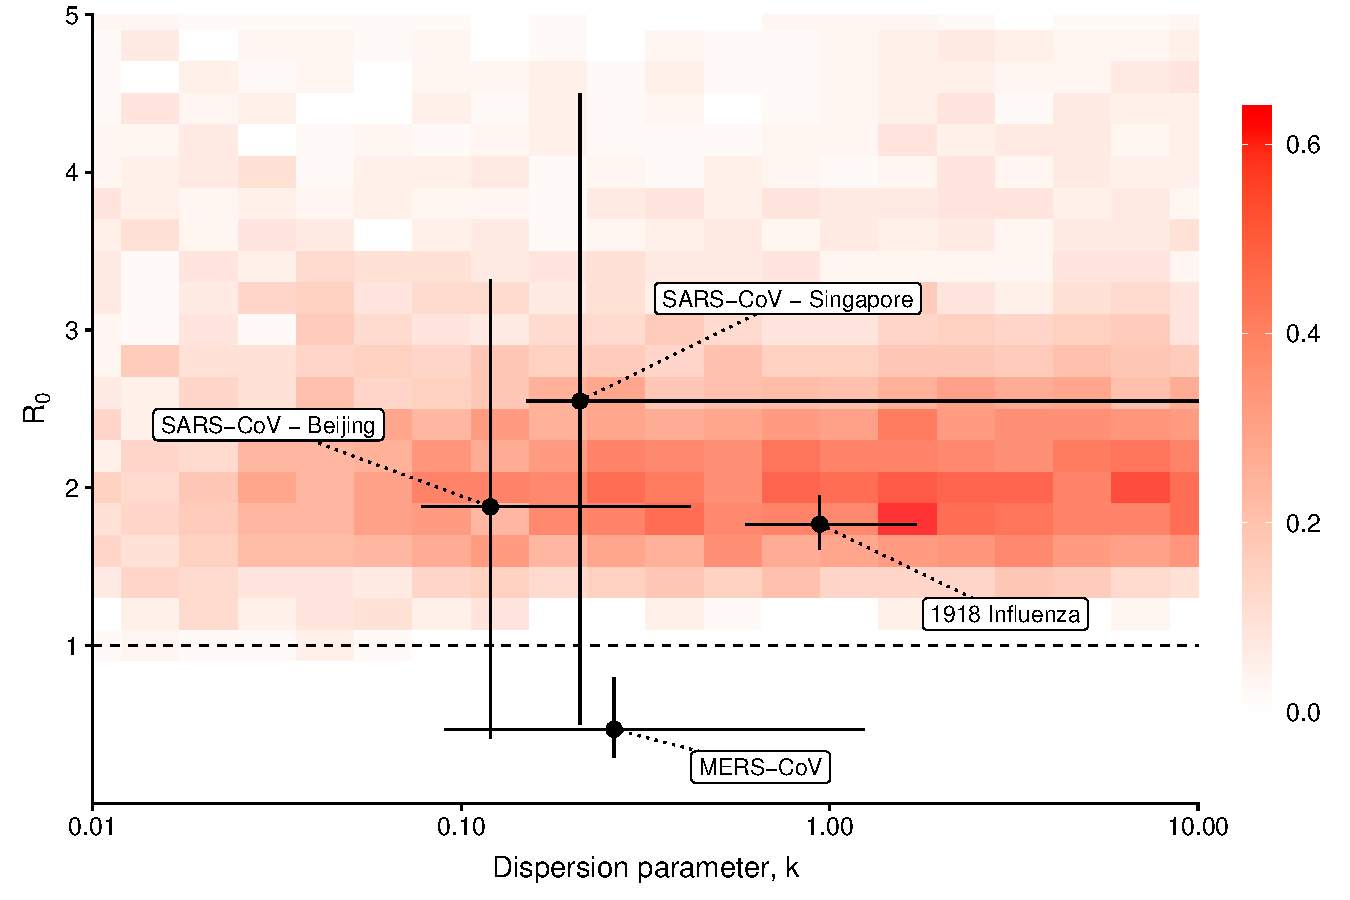
\includegraphics[width=.9\linewidth]{../figure/fig1.pdf}
	\caption{Proportion of simulated epidemics that lead to a cumulative incidence between 1000 and 9700 on January 18, 2020. This can be interpreted as the combinations of $R_0$ and $k$ values most compatible with epidemic data available on 2019-nCoV as of January 23, 2020, in comparison to the estimates of $R_0$ and $k$ for 2019-nCoV with corresponding parameters for the early human-to-human transmission of SARS-CoV in Singapore and Beijing, and of 1918-Influenza.\cite{Lloyd-Smith:2005,Fraser:2011,Kucharski:2015b}
	}
	\label{fig:fig1}
\end{figure}


\section*{Discussion}

After SARS-CoV in 2002 and of MERS-CoV in 2012, the emergence of 2019-nCoV in Wuhan, China rises a lot of concern worldwide.
An emergency WHO meeting on January 22, 2020 concluded that the lack of information about the patterns of transmission of the disease limited the ability of WHO to declare a public health emergency of international concern (PHEIC).\cite{whoreco}
The increasing research activity on 2019-nCoV has led to estimates of animal-to-human transmission,\cite{Chen2020.01.19.911669}, estimates of epidemic size using air travel data,\cite{Imai:2020, vespi:2020}, and a better characterization of the virological characteristics of the virus.\cite{Shi:2020}
This analysis is the first to focus on the quantification of early human-to-human transmission of 2019-nCoV.
The observed patterns of transmission confirm that the current situation has a much closer relationship to what was observed during the early stages of SARS-CoV transmission in Singapore and Beijing rather than during the emergence of MERS-CoV in the Middle-East.\cite{Lloyd-Smith:2005,Kucharski:2015b}
Although very different virological characteristics limit the relevance of the comparison, the transmission patterns of nCoV-2019 are also similar to those of 1918 influenza.

% lay summary
The scarcity of available data, especially on case counts by disease onset as well as contact tracing, greatly limits the precision of the estimates and does not allow for any reliable forecast of epidemic spread.
While based on few data points, this analysis still has the potential to bring to light important insights regarding human-to-human transmission.
First, our estimates of $R_0$ suggests that the disease has the potential for sustained human-to-human transmission.
This implies that important prevention and control measures will be crucial at this stage in order to stop the circulation of the virus.
The recent shutdown of the whole city of Wuhan shows that the Chinese authorities are well aware of the potential magnitude of the problem.
Second, it is not possible at the moment to ignore the risk of a superspreading event, but our analysis suggest that this risk is at worst of a similar magnitude as SARS-CoV and MERS-CoV.
This has important implications for international travel, as superspreading increases the risk of large clusters of infections in distant countries originating from one or a few unidentified imported cases.
This fact is in favour of a close monitoring of every passenger travelling from the Wuhan region of China, without excluding the possibility of long incubation periods.
The implementation of control measures in hospital settings, especially emergency rooms, will also be of prime importance, as has been shown by the examples of MERS-CoV in South Korea\cite{oh2015middle} and in Saudi Arabia.\cite{assiri2013hospital} 

% technical summary
Our analysis, while relatively crude, has two important strengths.
First, it is based on the simulation of a wide range of possibilities regarding the parameter values and allows for the full propagation of the many remaining uncertainties regarding 2019-nCoV and the situation in Wuhan: the size of the initial zoonotic event at the wet market, the date(s) of the initial animal-to-human transmission event(s) and the generation time interval.
While accounting for all these uncertainties, our analysis provides a reliable summary of the current state of knowledge about the human-to-human transmissibility of 2019-nCoV.
Second, its focus on the possibility of superspreading events by using negative-binomial offspring distributions is very important in the context of emerging coronaviruses.\cite{Lloyd-Smith:2005,Althaus:2015b}
While our estimate of $k$ remains very imprecise, our simulation suggests that lower values of $k$ (below 0.1), corresponding to a high risk of superspreading) are less likely than higher values (above 10), corresponding to a lower risk of superspreading.
It should however be reminded that values of $k$ in the range 0.1-0.2 are still compatible with the occurrence of large superspreading events, especially in hospital settings.\cite{oh2015middle,assiri2013hospital} 

% conclusion
Our analysis suggests that the early pattern of human-to-human transmission 2019-nCoV is reminiscent of SARS-CoV emergence in 2002.
Going forward, international collaboration and coordination will be crucial in order to contain the spread of 2019-nCoV.
As for previous emergences of coronaviruses, a particular attention should be given on the prevention of superspreading events, with important implications regarding screening and identification of imported cases among travellers, and on preventing transmission in hospital settings.
While it is likely that 2019-nCoV will continue to spread in the short-term, it should be reminded that control measures have been able to stop transmission in the past.
The relatively low case fatality ratio observed at this early stage also suggests that while 2019-nCoV might spread as much as SARS-CoV, it is unlikely to result in as many deaths.


\section{Acknowledgements}
JR is funded by the Swiss National Science Foundation (grant 174281).
\section{Conflict of interest}
None declared.

\section{Authors' contributions}

JR and CLA designed the study, JR performed model simulations, JR and CLA analyzed and interpreted the results and wrote the manuscript.

\bibliography{ncov.bib}
\bibliographystyle{unsrt}  
\end{document}
